\section{Compressed Sensing with Coordinate Descent}\label{cd}
First, let us look at the Coordinate Descent algorithm in its simplest form, and discuss its properties. With compressed sensing reconstructions, we want to find an image which is close to the measured Visibilities, but also has the smallest regularization penalty. In essence, we want to minimize the objective \eqref{cd:clean}, where the L2 term $\left \| V - F^{-1}x \right \|_2^2$ forces the image to represent the Visibilities $V$, and the regularization term $\left \| x \right \|_1$ forces the image to have as few non-zero pixels as possible. The parameter $\lambda$ represents our trade-off between reconstruction accuracy and regularization. 
 
\begin{equation}\label{cd:clean}
	\underset{x}{minimize} \: \left \| V - F^{-1}x \right \|_2^2 + \lambda \left \| x \right \|_1 \\
\end{equation}

The objective function \eqref{cd:clean} has a property, which we can exploit with Coordinate Descent: The optimum for a single pixel, if we keep all others fixed, turns out to be a parabola. The optimum for a single pixel of \eqref{cd:clean} is simply finding the apex of a parabola, followed by a shrink operation. Sadly, the pixels are not independent of each other, we need to iterate over each pixels several times until the solution converges. This leads to the following optimization algorithm, written in python code:

\begin{lstlisting} 
def coordinate_descent(V_residual, x, lambda, max_iter):
	for k in range(0, max_iter):
		for i in pixels_row:
			for j in pixels_column:
				x_old = x[i, j]
				fourier_column = calculate_fourier_transform(i, j)
				fr = real(fourier_column)
				fi = imag(fourier_column)
				rr = real(V_residual)
				ri = imag(V_residual)
				
				#find apex
				a = sum(fr**2 + 2*fr*fi + fi**2)
				b = sum(fr*rr + fr*ri + fi*rr + fi*ri)
				x_new = b / a + x_old
				
				x_new = shrink(x_new, lambda)
				x[i, j] = x_new
				V_residual = V_residual - fourier_column * (x_new - x_old)
\end{lstlisting}\label{cd:basic}

This algorithm calulates the whole Fourier Transform Matrix $F^{-1}$. But we do not need any approximation algorithms like the non-uniform FFT, and we can handle the $w$-term easily.

We do not need to iterate over all pixels, only those that are likely to be non-zero. Convergence in general hard to prove, but in practice has been shown to work well enough. Turns out to be robust for paralellism

Heuristic heaven

We use the starlet transform \eqref{cd:starlet}

$x = D\alpha$

\begin{equation}\label{cd:starlet}
\underset{x}{minimize} \: \left \| V - F^{-1}D\alpha \right \|_2^2 + \lambda \left \| \alpha \right \|_1 \\
\end{equation}




\subsection{Starlet Transform} \label{cd:starlets}
Starlet is a multi-scale wavelet representation which were specifically developed for astronomy.

Over-complete representation. More starlets than there are pixels. Sparse representation, the number of non-zero starlets is smaller than the number of pixels

Starlets as a series of convolutions.

Forward transform, from image to starlets

From Starlets to image

\subsection{Active set heuristic with Starlets}\label{cd:heuristic}
Even though the starlets are an over-complete dictionary, they have an approximate transform from image to starlet space. For Coordinate Descent, this can be used as a active set heuristic: We try to find the coefficients which are likely to be non-zero. This helps us so we do not need to calculate the whole matrix product $F^{-1}D$. We only use columns that are likely to be not zero.

\begin{figure}[h]
	\centering
	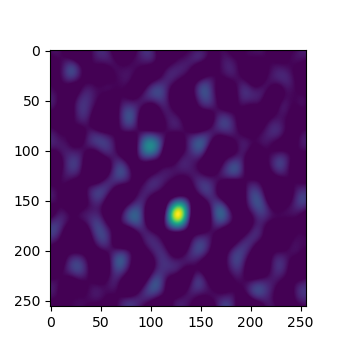
\includegraphics[width=0.5\linewidth]{./chapters/05.algorithms/sim02/starlets0.png}
	\caption{Starlet Level 0}
	\label{alg:heuristic:starlet}
\end{figure}

The higher the number, the more likely this component is to be non-zero. It is essentially a probability distribution for which starlet components are non-zero.

Stupid approach with line search. Could be done more efficiently by using the histogram of the starlet level.

\subsection{Implementation}
coordinate descent with active set heuristic

